\chapter{Npovedovanje}
\label{ch:text-napovedovanje}

Do sedaj smo napovedovali samo ozanke, ki smo jih že poznali - tip posamezne pravljice. Pravilne odgovore smo že imeli podane v stolpcu ATU Topic. Kaj pa če nimamo te informacije? Bi lahko napovedali tip pravljice za neoznačeno besedilo?

\begin{figure}[h]
    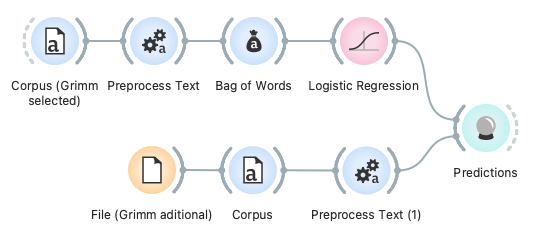
\includegraphics[width=\linewidth]{napovedovanje-workflow.png}%
    \caption{ }
    \label{fig:002-preprocess}
\end{figure}

Odprite nov gradnik File in v polje URL prekopirajte naslov \url{https://file.biolab.si/datasets/grimm-tales-additional.tab}. Na ta način boste naložili manjšo zbirko Grimmovih pravljic, ki niso v originalnem korpusu na katerem se je model učil. Z gradnikom Corpus pretvorite zbirko v kropus. Poglejte jih v gradniku Corpus Viewer in poskusite sami ugotoviti tip pravljice.
Sedaj povežite gradnik Predictions enako kot prej - logistična regresija naj pošilja zgrajen model, nov gradnik Corpus pa naj pošilja podatke za napovedi (ne pozabite novega korpusa predhodno še predprocesirati). Logistična regresija pravi, da sta dve pravljici magični, dve pa živalski.
The Fox and the Horse je napovedana kot živalska pravljica? Sliši se kar prav!

\begin{figure*}[h]
    \centering
    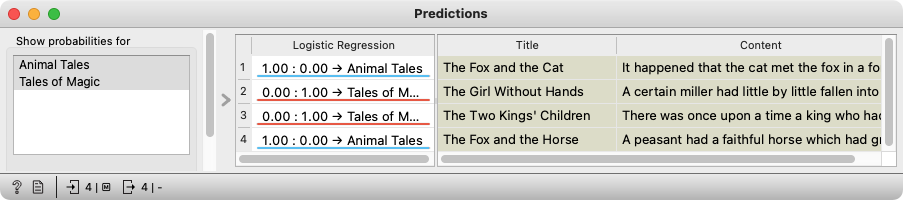
\includegraphics[width=\linewidth]{napovedovanje-predictions.png}%
    \caption{}
    \label{fig:002-word-cloud}
\end{figure*}